\documentclass[tikz]{standalone}
\usetikzlibrary{calc,trees,positioning,arrows,chains,shapes.geometric,%
    decorations.pathreplacing,decorations.pathmorphing,shapes,%
    matrix,shapes.symbols,shapes.arrows,fit}

\pgfdeclarelayer{back}
\pgfsetlayers{back,main}

\makeatletter
\tikzset{
  fitting node/.style={
    inner sep=0pt,
    fill=none,
    draw=none,
    reset transform,
    fit={(\pgf@pathminx,\pgf@pathminy) (\pgf@pathmaxx,\pgf@pathmaxy)}
  },
  reset transform/.code={\pgftransformreset}
}
\makeatother


\begin{document}
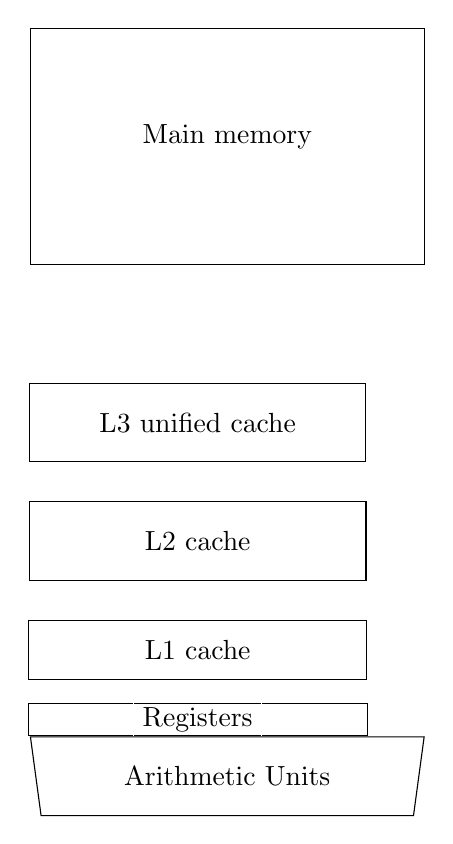
\begin{tikzpicture}
  \draw (0,0) rectangle (5,3) node[fitting node] (RAM) {Main memory};
  \node (RAM_right_offset) [coordinate] at($(RAM.south east)!.3!(RAM.south)$) {};
  \node (RAM_left_offset) [coordinate] at($(RAM.south west)!.5!(RAM.south)$) {};


  
  \draw ([yshift=-1.5cm]RAM.south west) rectangle ([yshift=-2.5cm]RAM_right_offset) node[fitting node,align=center] (l3cache) {};
  \node (l3cache_label) [draw=white] at(l3cache) {L3 unified cache};
  \draw ([yshift=-.5cm]l3cache.south west) rectangle ([yshift=-1.5cm]l3cache.south east) node[fitting node,align=center] (l2cache) {};
  \node (l2cache_label) [draw=white] at(l2cache) {L2 cache};
  
  \draw ([yshift=-.5cm]l2cache.south west) rectangle ([yshift=-1.25cm]l2cache.south east) node[fitting node,align=center] (l1cache) {};
  \node (l1cache_label) [draw=white] at(l1cache) {L1 cache};
  
  \draw ([yshift=-.3cm]l1cache.south west) rectangle ([yshift=-.7cm]l1cache.south east) node[fitting node,align=center] (registers) {};
  \node (regs_label) [draw=white] at(registers) {Registers};

  \node (cpu) [trapezium,draw,minimum width=5cm,minimum height=1cm, trapezium stretches body,rotate=180]
at ([yshift=-8.cm]RAM) {};
  \node (cpu_label) [draw=white] at(cpu) {Arithmetic Units};

  
  \end{tikzpicture}
\end{document}
